%\documentclass[a4,semhelv,landscape]{seminar}
\documentclass[landscape]{slides}
%\documentclass[pdf, default, slideBW, nocolorBG]{prosper}
\usepackage[left=0.2cm,top=0.2cm,right=0.2cm,bottom=0.2cm,nohead,nofoot]{geometry}
%\def\everyslide{\sffamily}
%\usepackage{fullpage}
\usepackage{graphicx}
\usepackage[usenames]{color}
%\usepackage{color}
\usepackage{verbatim}
\usepackage{nopageno}
\usepackage{setspace}
%\usepackage{times}
% define some nice colors
\definecolor{myred}{rgb}{0.6,0,0}
\definecolor{myblue}{rgb}{0,0.2,0.4}
\definecolor{mygreen}{rgb}{0,0.5,0.0}
\definecolor{mypurple}{cmyk}{0.5,1.0,0.0,0.0}
\definecolor{myorange}{cmyk}{0.0,0.75,1.0,0.0}
%\color{myblue}

\begin{document}
%%%%%%%%%%%%%%%%%%%%%%%%%%%%%%%%%%%%%%%%%%%%%%%%%%%%%%%%%%%%%%%%%%%%
%Slide 0 - title
\begin{slide}
\begin{center}
\large{\textbf{Reference-guided annotation of viral genomes}}

\normalsize

Eric Nawrocki \\

\medskip

\medskip

\medskip

\medskip

\medskip

\small
\begin{tabular}{c}
%Alejandro Sch\"{a}ffer's group \\
%\\
National Center for Biotechnology Information\\
National Institutes of Health\\
\\
\end{tabular}

\vspace{0.1in}

\includegraphics[width=2.5in]{figs/ncbi-logo}

\end{center}
\end{slide}
%%%%%%%%%%%%%%%%%%%%%%%%%%%%%%%%%%%%%%%%%%%%%%%%%%%%%%%%%%%%%%%%%%%%%%
\begin{slide}
\begin{center}

\textbf{Most prevalent viral genomes in GenBank\footnote{Current as of March, 2018.}}

\tiny
\begin{tabular}{r|l|r|l|l|l|r|r}
     &                     &              &                &          &        &       & \#mature \\ 
rank & species             & \#seqs       & family         & type     & host   &  \#CDS& peptides \\ \hline
     &                     &              &                &          &        &       &          \\ 
  1  &  Influenza          &   503,115    & Orthomyxoviridae& (-)ssRNA& humans+&    11 & -        \\ %NC_007370
     &                     &              &                &          &        &       &          \\ 
  2  & Rotavirus A         &58,405\footnote{sum of 11 segments}& Reoviridae&dsRNA&humans&   12 & -\\ %NC_011503
     &                     &              &                &          &        &       &          \\ 
  3  & Hepatitis B         &         9211 & Hepadnaviridae & dsDNA-RT & humans &     7 & -        \\ %NC_003977
     &                     &              &                &          &        &       &          \\ 
  4  & Dengue              &         4853 & Flaviviridae   & (+)ssRNA & humans &     1 & 14       \\ %NC_001477
     &                     &              &                &          &        &       &          \\ 
  5  & HIV-1               &        2597  & Retroviridae   & ssRNA-RT & humans &    10 & 14       \\ %NC_001802
     &                     &              &                &          &        &       &          \\ 
  6  & Hepatitis C         &        2185  & Flaviviridae   & (+)ssRNA & humans &     2 & 10       \\ %NC_004102
     &                     &              &                &          &        &       &          \\ 
  7  & Porcine circovirus  &        1905  & Circoviridae   & ssDNA    & pigs   &     3 & -        \\ %NC_005148
     &                     &              &                &          &        &       &          \\ 
  8  & West Nile           &        1667  & Flaviviridae   & (+)ssRNA & humans &     3 & 16       \\ %NC_009942
     &                     &              &                &          &        &       &          \\ 
  9  & Ebola               &        1384  & Flaviviridae   & (+)ssRNA & humans &     9 & -        \\ %NC_002549
     &                     &              &                &          &        &       &          \\ 
 10  & Enterovirus A       &        1222  & Picarnoviridae & (+)ssRNA & humans &     1 & 11       \\ %NC_001612
     &                     &              &                &          &        &       &          \\ 
 11  & RSV                 &        1122  & Orthopneumovirus& (-)ssRNA& humans &    11 & -        \\ %NC_001781
     &                     &              &                &          &        &       &          \\ 
 12  & Norwalk virus       &        1009  & Calciviridae   & (+)ssRNA & humans &     3 & 6        \\ %NC_029646
     &                     &              &                &          &        &       &          \\ 
 13  & Maize streak virus  &         884  & Geminiviridae  & ssDNA    & plants &     4 & -        \\ %NC_001346
     &                     &              &                &          &        &       &          \\ 
 14  & Rabies lyssavirus   &         826  & Rhabdoviridae  & (-)ssRNA & humans+&     5 & -        \\ %NC_001542
     &                     &              &                &          &        &       &          \\ 
 15  & Enterovirus C       &         765  & Picarnoviridae & (+)ssRNA & humans &     1 & 13       \\ %NC_002058
\end{tabular}

\tiny
\flushright{$\dagger$ sum of 11 segments}
\vfill

\end{center}
\end{slide}
%%%%%%%%%%%%%%%%%%%%%%%%%%%%%%%%%%%%%%%%%%%%%%%%%%%%%%%%%%%%%%%%%%%%%%
\begin{slide}
\begin{center}
\textbf{The Virus Variation Resource is a powerful tool for viral research}

\begin{minipage}[c]{4in}
\tiny
\begin{itemize}
\item value added database that includes annotations not in GenBank
\item allows users to: 
\begin{itemize}
  \item select subsets of data based on desired criteria
    (host, country, gene, etc.)
  \item download alignments
  \item  compute trees
  \item  more...
\end{itemize}
\end{itemize}
\vfill
\end{minipage}
\begin{minipage}[c]{6in}
\includegraphics[width=6in]{figs/viv-page1}
\vfill
\end{minipage}

\vfill
\end{center}
\end{slide}
%%%%%%%%%%%%%%%%%%%%%%%%%%%%%%%%%%%%%%%%%%%%%%%%%%%%%%%%%%%%%%%%%%%%%%
\begin{slide}
\begin{center}
\textbf{The Virus Variation Resource is a powerful tool for viral research}

\includegraphics[width=8.5in]{figs/viv-dengue-query}

\vfill
\end{center}
\end{slide}
%%%%%%%%%%%%%%%%%%%%%%%%%%%%%%%%%%%%%%%%%%%%%%%%%%%%%%%%%%%%%%%%%%%%%%
\begin{slide}
\begin{center}
\textbf{Our initial goal was to develop an annotation pipeline to \\ benefit Virus Variation}

\small
\begin{itemize}
\item general method for annotating existing and new viral genome
  sequences for a species using trusted annotation for that species (e.g. RefSeq)
\item identify interesting characteristics that Virus Variation can
  allow users to sort/select based on:
\begin{itemize}
  \item identification of high quality sequences that meet specific expectations
  \item identification of sequences that deviate from expectations in
    various ways
    \begin{itemize}
      \item early stop codon
      \item above or below a specific fractional identity to reference 
      \item more...
    \end{itemize}
\end{itemize}
\end{itemize}

\normalsize
\textbf{A new goal is to use this annotation pipeline to validate/annotate incoming submissions of sequences from commonly deposited viruses} 

\small
\begin{itemize}
\item use unexpected features identified by pipeline to flag issues for indexers and submitters to deal with
\item currently testing on Norovirus, and soon to be testing on Ebolavirus
\end{itemize}

\end{center}
\vfill
\end{slide}
%%%%%%%%%%%%%%%%%%%%%%%%%%%%%%%%%%%%%%%%%%%%%%%%%%%%%%%%%%%%%%%%%%%%%%
\begin{slide}
\begin{center}

\textbf{Four pilot species were chosen from the 15 most prevalent}

\textbf{Most prevalent viral genomes in GenBank\footnote{Current as of March, 2018.}}


\tiny
\begin{tabular}{r|l|r|l|l|l|r|r}
     &                     &              &                &          &        &       & \#mature \\ 
rank & species             & \#seqs       & family         & type     & host   &  \#CDS& peptides \\ \hline
     &                     &              &                &          &        &       &          \\ 
  1  & Influenza           &   503,115    & Orthomyxoviridae& (-)ssRNA& humans+&    11 & -        \\ %NC_007370
     &                     &              &                &          &        &       &          \\ 
  2  & Rotavirus A         &58,405\footnote{sum of 11 segments}& Reoviridae&dsRNA&humans&   12 & -\\ %NC_011503
     &                     &              &                &          &        &       &          \\ 
  \textcolor{myorange}{3}  & \textcolor{myorange}{Hepatitis B}         &         \textcolor{myorange}{9211} & \textcolor{myorange}{Hepadnaviridae} & \textcolor{myorange}{dsDNA-RT} & \textcolor{myorange}{humans} &     \textcolor{myorange}{7} & \textcolor{myorange}{-}        \\ %NC_003977
     &                     &              &                &          &        &       &          \\ 
  \textcolor{myorange}{4}  & \textcolor{myorange}{Dengue}              &         \textcolor{myorange}{4853} & \textcolor{myorange}{Flaviviridae}   & \textcolor{myorange}{(+)ssRNA} & \textcolor{myorange}{humans} &     \textcolor{myorange}{1} & \textcolor{myorange}{14}       \\ %NC_001477
     &                     &              &                &          &        &       &          \\ 
  5  & HIV-1               &        2597  & Retroviridae   & ssRNA-RT & humans &    10 & 14       \\ %NC_001802
     &                     &              &                &          &        &       &          \\ 
  6  & Hepatitis C         &        2185  & Flaviviridae   & (+)ssRNA & humans &     2 & 10       \\ %NC_004102
     &                     &              &                &          &        &       &          \\ 
  7  & Porcine circovirus  &        1905  & Circoviridae   & ssDNA    & pigs   &     3 & -        \\ %NC_005148
     &                     &              &                &          &        &       &          \\ 
  \textcolor{myorange}{8}  & \textcolor{myorange}{West Nile}           &        \textcolor{myorange}{1667}  & \textcolor{myorange}{Flaviviridae}   & \textcolor{myorange}{(+)ssRNA} & \textcolor{myorange}{humans} &     \textcolor{myorange}{3} & \textcolor{myorange}{16}       \\ %NC_009942
     &                     &              &                &          &        &       &          \\ 
  9  & Ebola               &        1384  & Flaviviridae   & (+)ssRNA & humans &     9 & -        \\ %NC_002549
     &                     &              &                &          &        &       &          \\ 
 10  & Enterovirus A       &        1222  & Picarnoviridae & (+)ssRNA & humans &     1 & 11       \\ %NC_001612
     &                     &              &                &          &        &       &          \\ 
 11  & RSV                 &        1122  & Orthopneumovirus& (-)ssRNA& humans &    11 & -        \\ %NC_001781
     &                     &              &                &          &        &       &          \\ 
 12  & Norwalk virus       &        1009  & Calciviridae   & (+)ssRNA & humans &     3 & 6        \\ %NC_029646
     &                     &              &                &          &        &       &          \\ 
\textcolor{myorange}{13}  & \textcolor{myorange}{Maize streak virus}  &         \textcolor{myorange}{884}  & \textcolor{myorange}{Geminiviridae}  & \textcolor{myorange}{ssDNA}    & \textcolor{myorange}{plants} &     \textcolor{myorange}{4} & \textcolor{myorange}{-}        \\ %NC_001346
     &                     &              &                &          &        &       &          \\ 
 14  & Rabies lyssavirus   &         826  & Rhabdoviridae  & (-)ssRNA & humans+&     5 & -        \\ %NC_001542
     &                     &              &                &          &        &       &          \\ 
 15  & Enterovirus C       &         765  & Picarnoviridae & (+)ssRNA & humans &     1 & 13       \\ %NC_002058
\end{tabular}

\tiny
\flushright{$\dagger$ sum of 11 segments}
\vfill
\end{slide}
%%%%%%%%%%%%%%%%%%%%%%%%%%%%%%%%%%%%%%%%%%%%%%%%%%%%%%%%%%%%%%%%%%%%%%
%%%%%%%%%%%%%%%%%%%%%%%%%%%%%%%%%%%%%%%%%%%%%%%%%%%%%%%%%%%%%%%%%%%%%%
\begin{slide}
\begin{center}
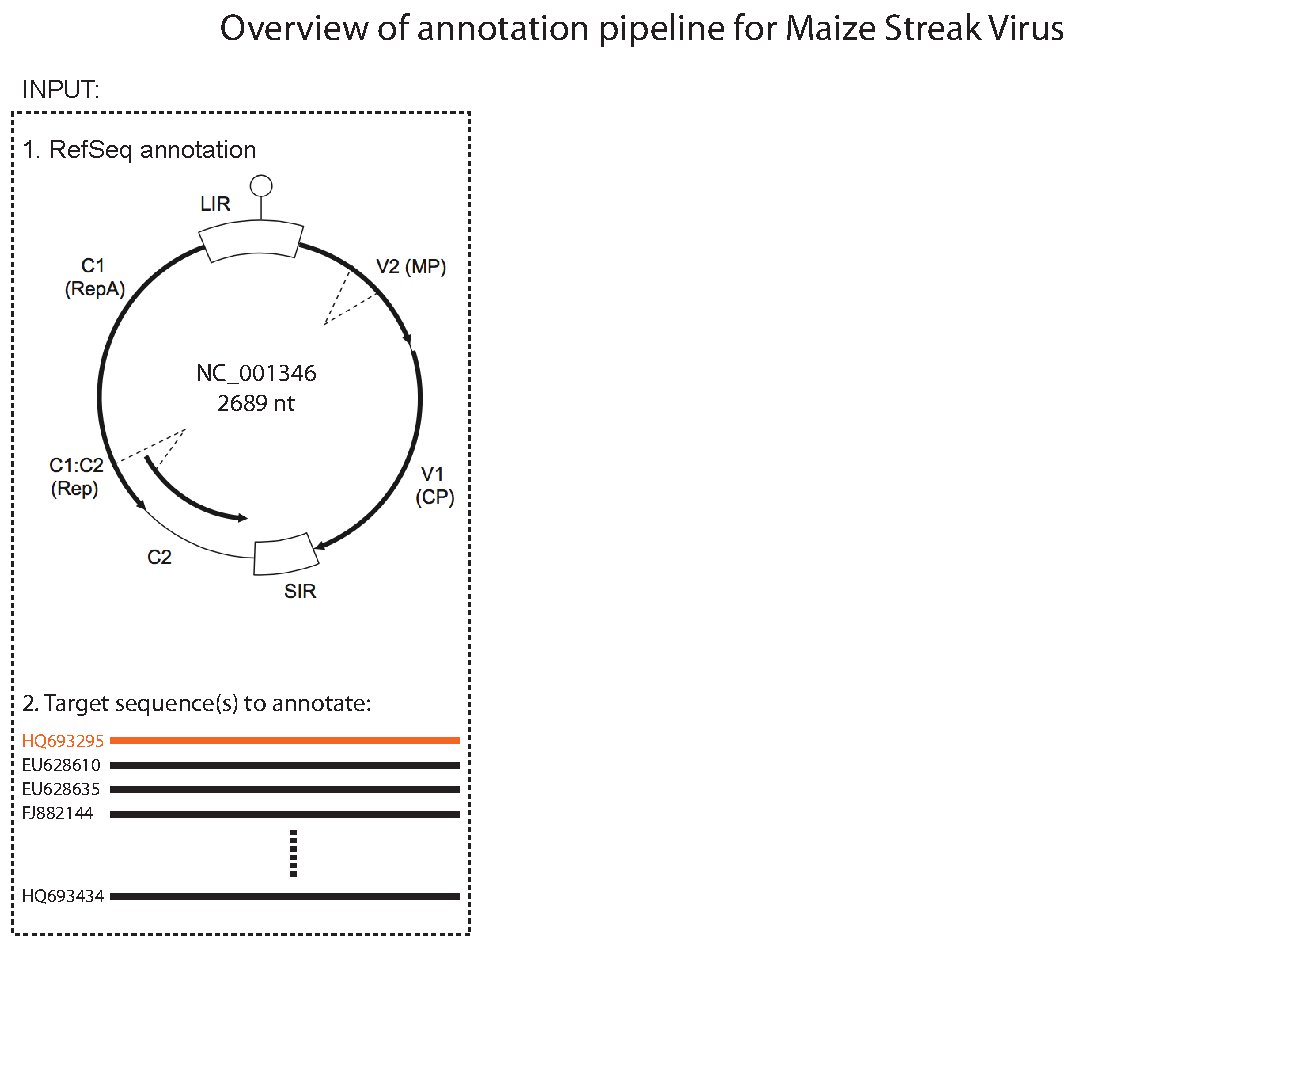
\includegraphics[width=10in]{figs/annotation-schematic-msv-1}
\end{center}
\vfill
\end{slide}
%%%%%%%%%%%%%%%%%%%%%%%%%%%%%%%%%%%%%%%%%%%%%%%%%%%%%%%%%%%%%%%%%%%%%%
\begin{slide}
\begin{center}
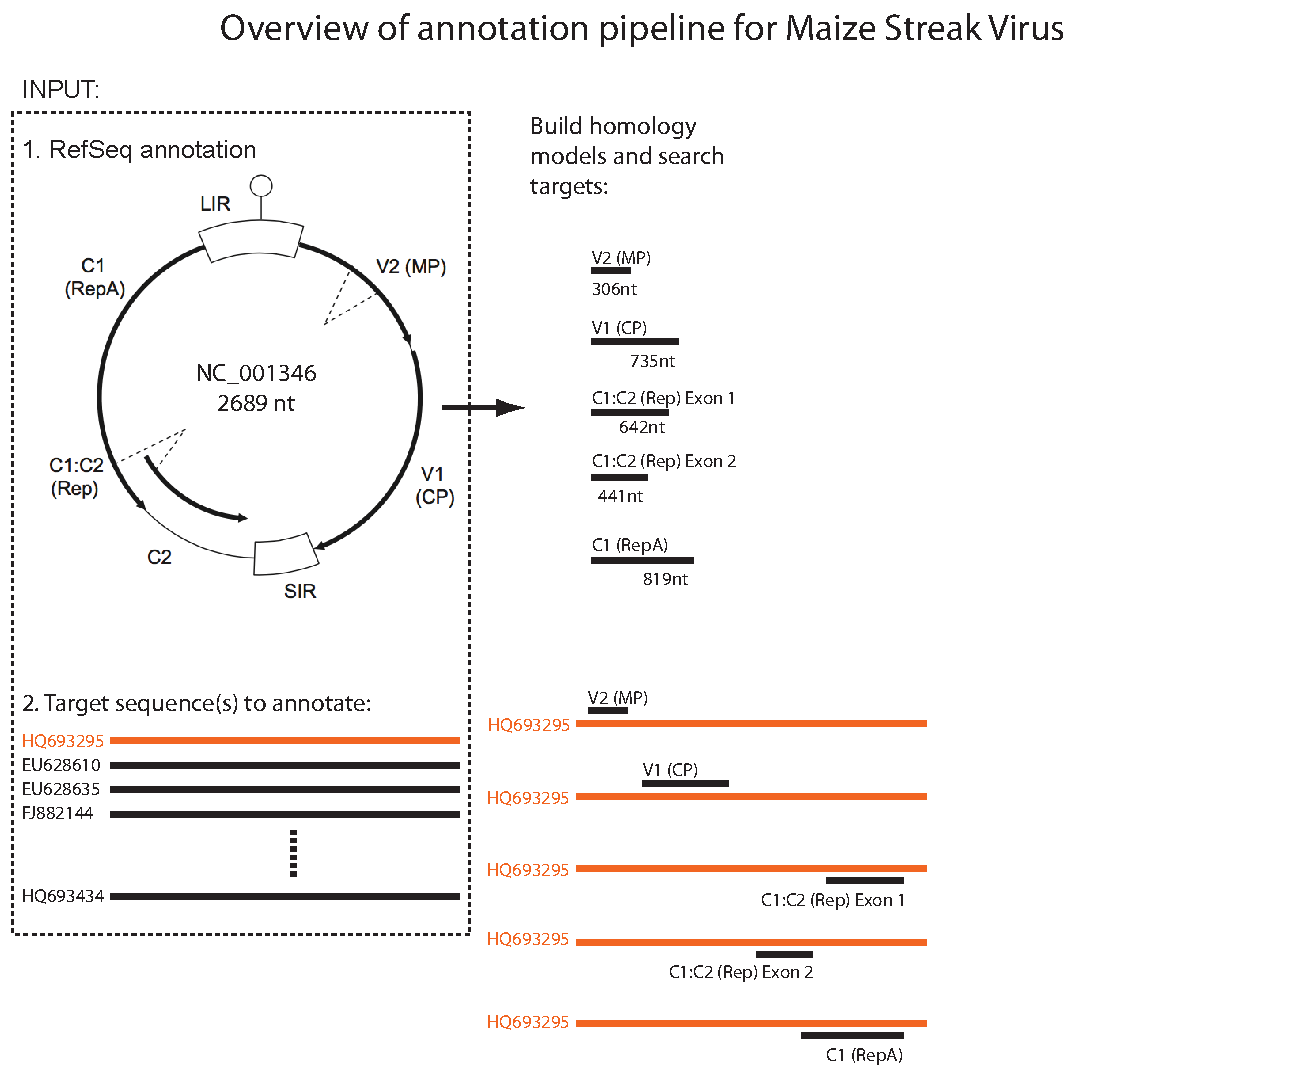
\includegraphics[width=10in]{figs/annotation-schematic-msv-2}
\end{center}
\vfill
\end{slide}
%%%%%%%%%%%%%%%%%%%%%%%%%%%%%%%%%%%%%%%%%%%%%%%%%%%%%%%%%%%%%%%%%%%%%%
\begin{slide}
\begin{center}
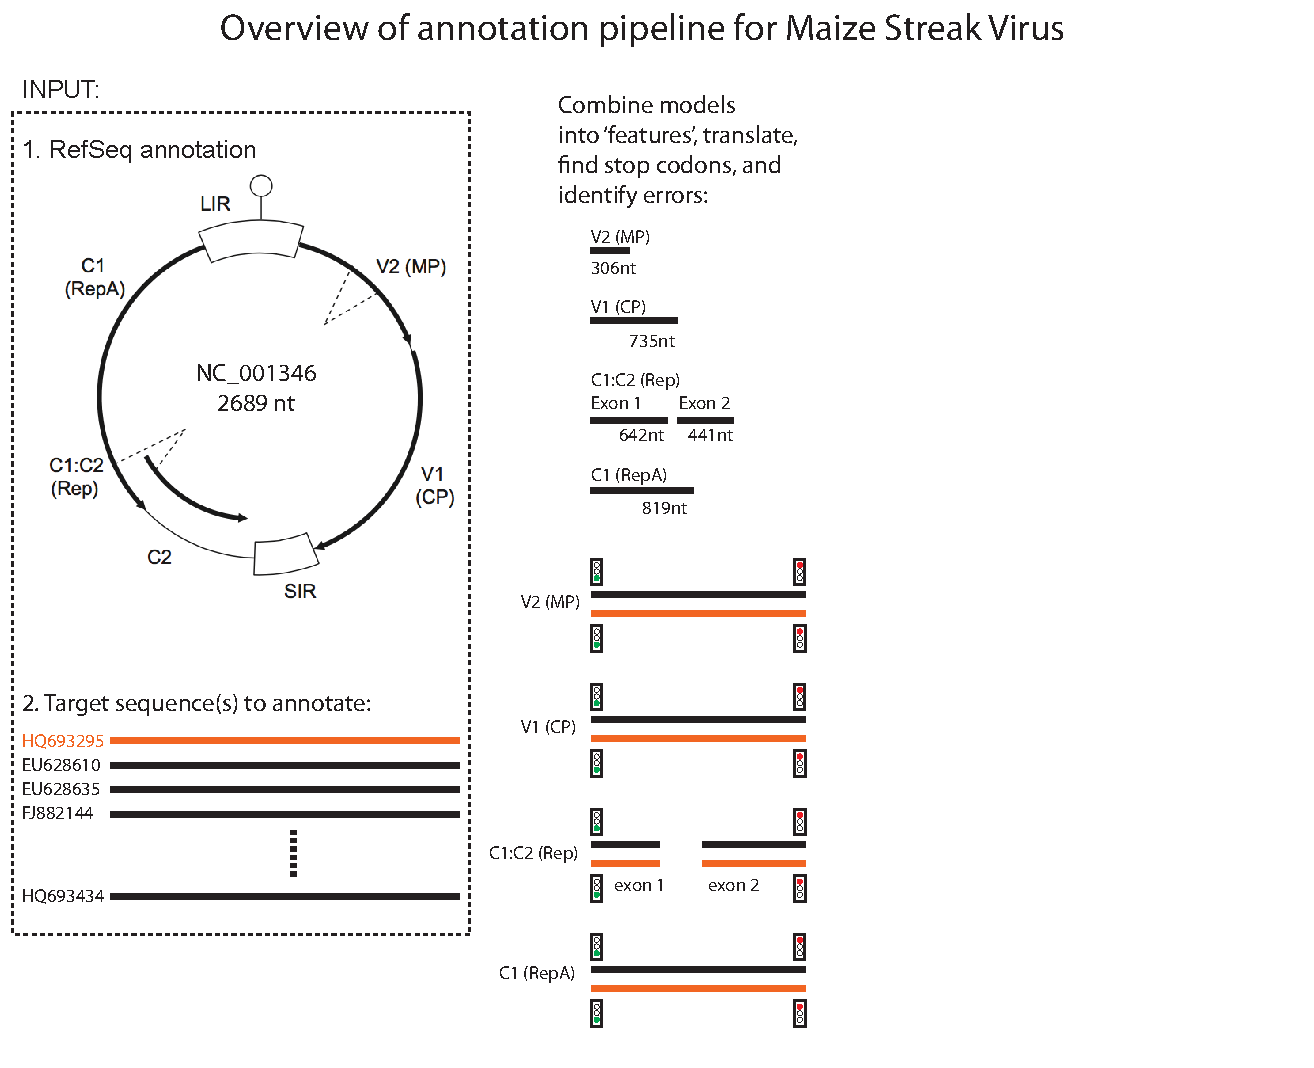
\includegraphics[width=10in]{figs/annotation-schematic-msv-3}
\end{center}
\vfill
\end{slide}
%%%%%%%%%%%%%%%%%%%%%%%%%%%%%%%%%%%%%%%%%%%%%%%%%%%%%%%%%%%%%%%%%%%%%%
\begin{slide}
\begin{center}
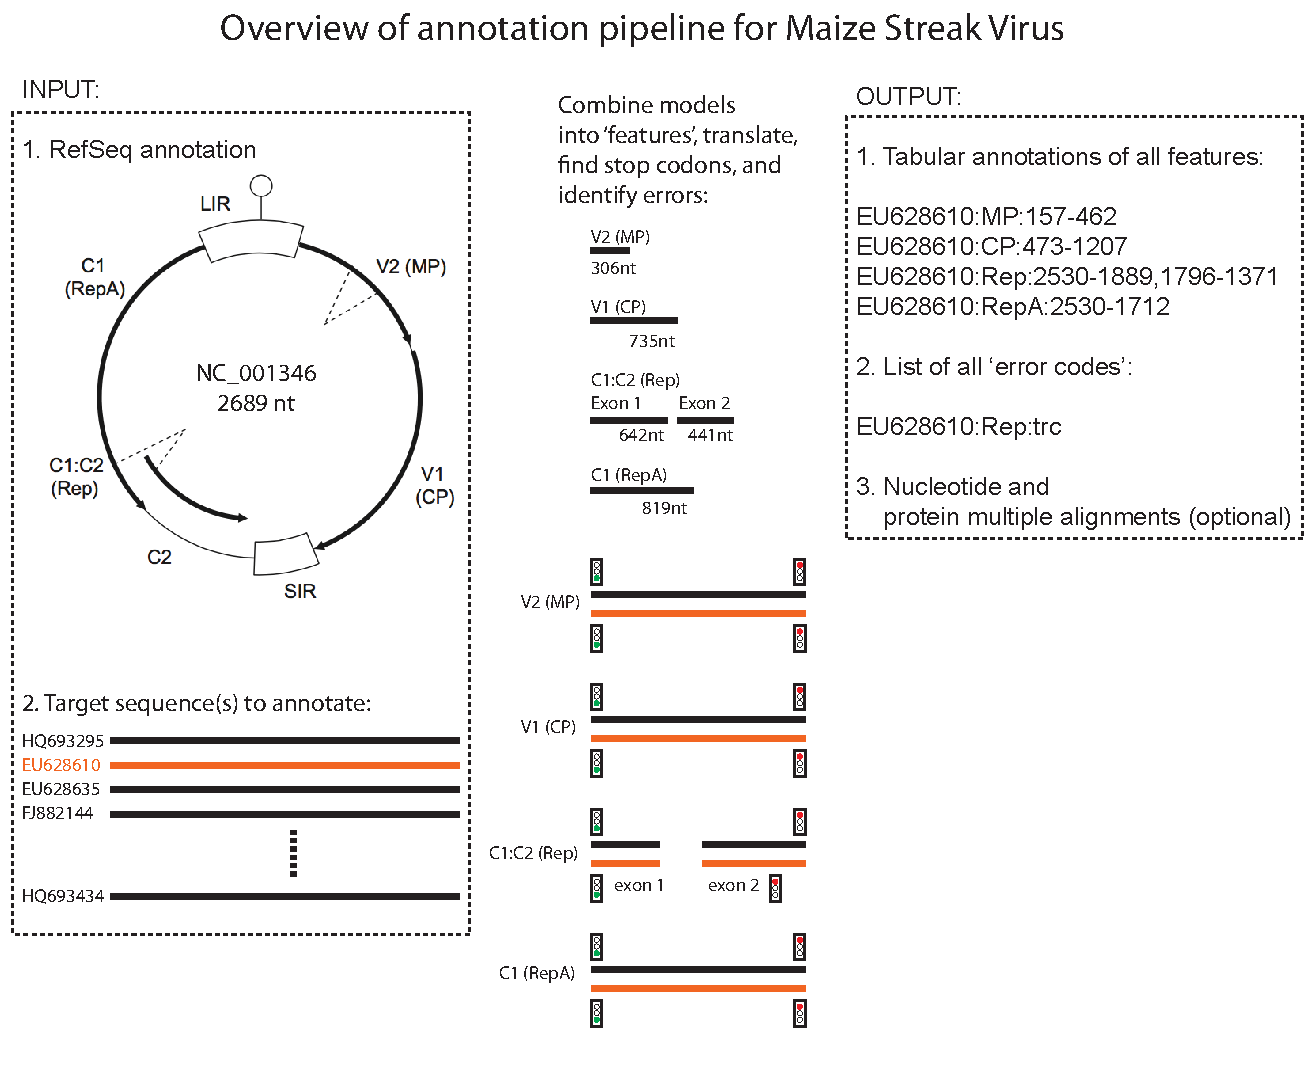
\includegraphics[width=10in]{figs/annotation-schematic-msv-4}
\end{center}
\vfill
\end{slide}
%%%%%%%%%%%%%%%%%%%%%%%%%%%%%%%%%%%%%%%%%%%%%%%%%%%%%%%%%%%%%%%%%%%%%%
\begin{slide}
\begin{center}
\includegraphics[width=10in]{figs/annotation-schematic-dengue-1}
\end{center}
\vfill
\end{slide}
%%%%%%%%%%%%%%%%%%%%%%%%%%%%%%%%%%%%%%%%%%%%%%%%%%%%%%%%%%%%%%%%%%%%%%
\begin{slide}
\begin{center}
\includegraphics[width=10in]{figs/annotation-schematic-dengue-2}
\end{center}
\vfill
\end{slide}
%%%%%%%%%%%%%%%%%%%%%%%%%%%%%%%%%%%%%%%%%%%%%%%%%%%%%%%%%%%%%%%%%%%%%%
\begin{slide}
\begin{center}
\includegraphics[width=10in]{figs/annotation-schematic-dengue-3}
\end{center}
\vfill
\end{slide}
%%%%%%%%%%%%%%%%%%%%%%%%%%%%%%%%%%%%%%%%%%%%%%%%%%%%%%%%%%%%%%%%%%%%%%
\begin{slide}
\begin{center}
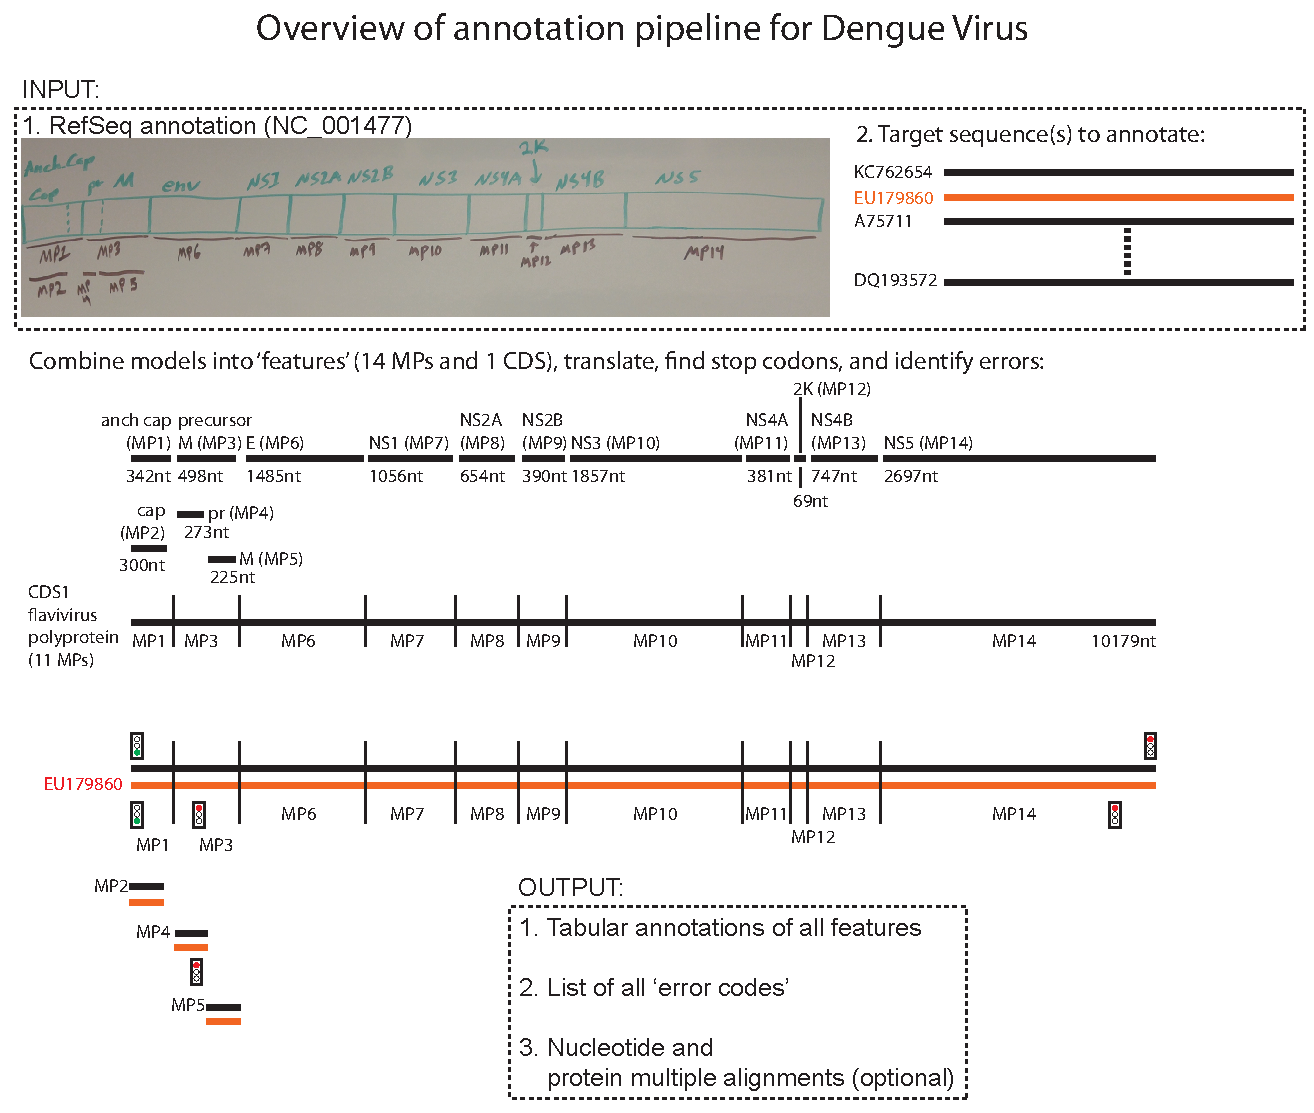
\includegraphics[width=10in]{figs/annotation-schematic-dengue-4-with-output}
\end{center}
\vfill
\end{slide}
%%%%%%%%%%%%%%%%%%%%%%%%%%%%%%%%%%%%%%%%%%%%%%%%%%%%%%%%%%%%%%%%%%%%%%
\begin{slide}
\begin{center}
\textbf{Error codes: 17 abnormal situations}

\small
\begin{itemize}
\item Per-feature (e.g. CDS, mature peptide) errors:
\begin{itemize}
\item Unexpected stop codon errors (trc, ext, nst, ntr)
\item Missing expected features (str, stp, nm3)
\item Problem with homology search prediction (bd5, bd3, nop)
\item Unexpected relationship to other features (olp, aja, ajb)
\item Problem annotating CDS due to mature peptide errors (aji, int, inp)
\end{itemize}
\item Per-sequence errors:
\begin{itemize} 
\item Lack of exactly one origin sequence (ori)
\end{itemize}
\end{itemize}

\end{center}
\vfill
\end{slide}
%%%%%%%%%%%%%%%%%%%%%%%%%%%%%%%%%%%%%%%%%%%%%%%%%%%%%%%%%%%%%%%%%%%%%%
\begin{slide}
\begin{center}
\textbf{trc error code reports a truncation due to an early stop codon}
\vspace{0.5in}

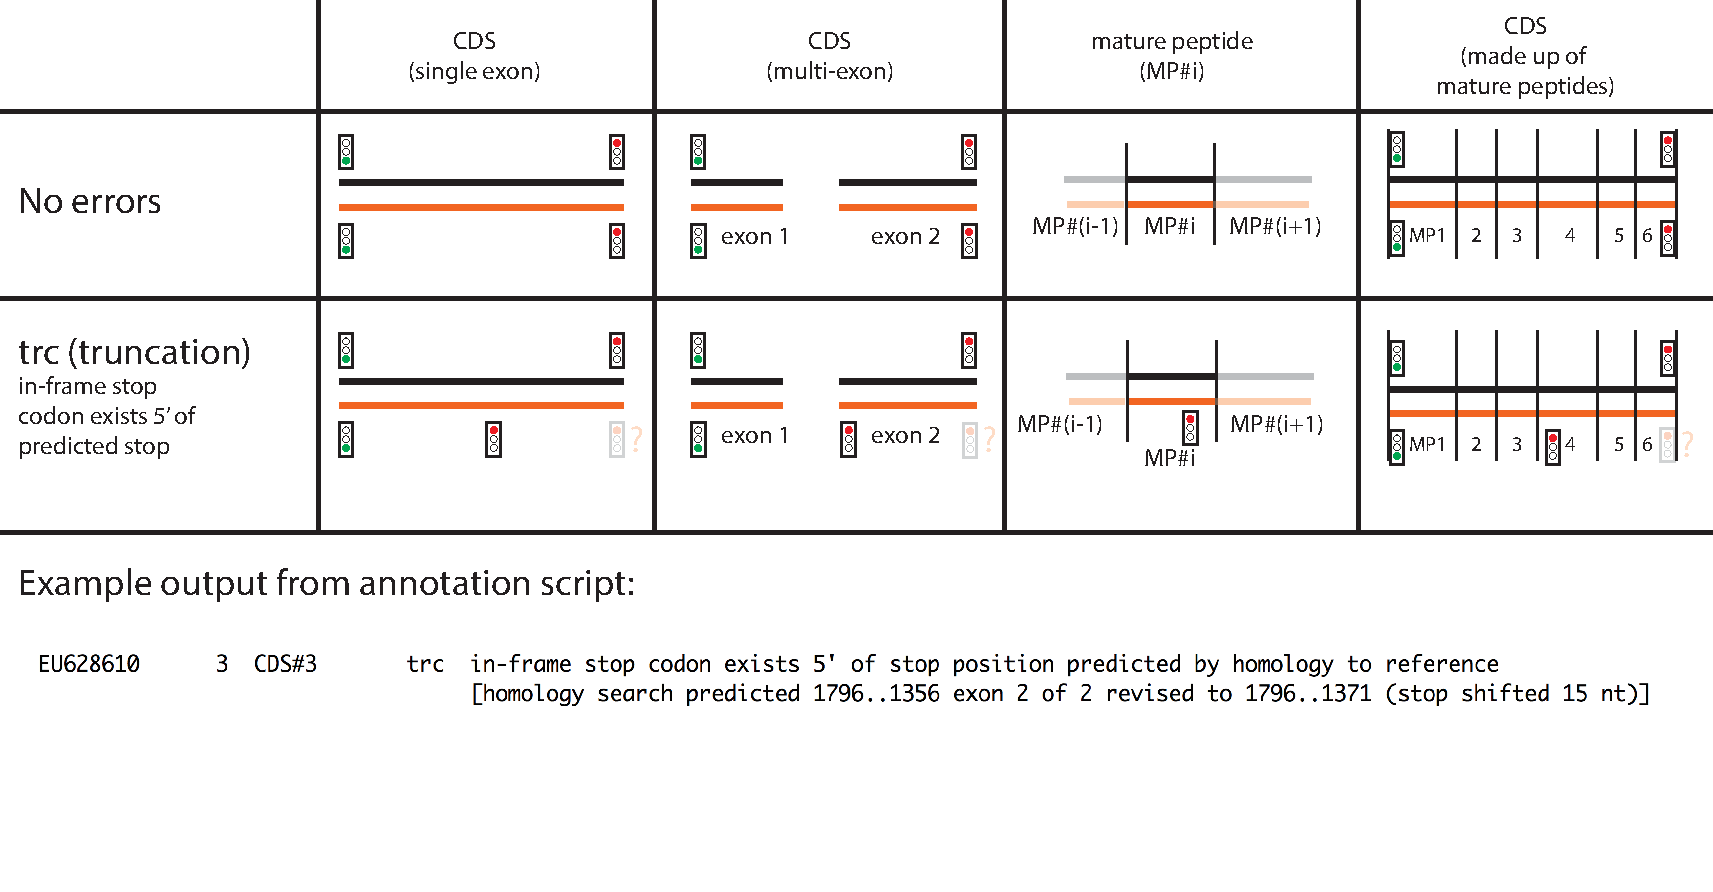
\includegraphics[width=10in]{figs/errornew-1-trc}
\end{center}
\vfill
\end{slide}
%%%%%%%%%%%%%%%%%%%%%%%%%%%%%%%%%%%%%%%%%%%%%%%%%%%%%%%%%%%%%%%%%%%%%%
\begin{slide}
\begin{center}
\textbf{ext: extended feature due to a missing stop codon}
\vspace{0.5in}

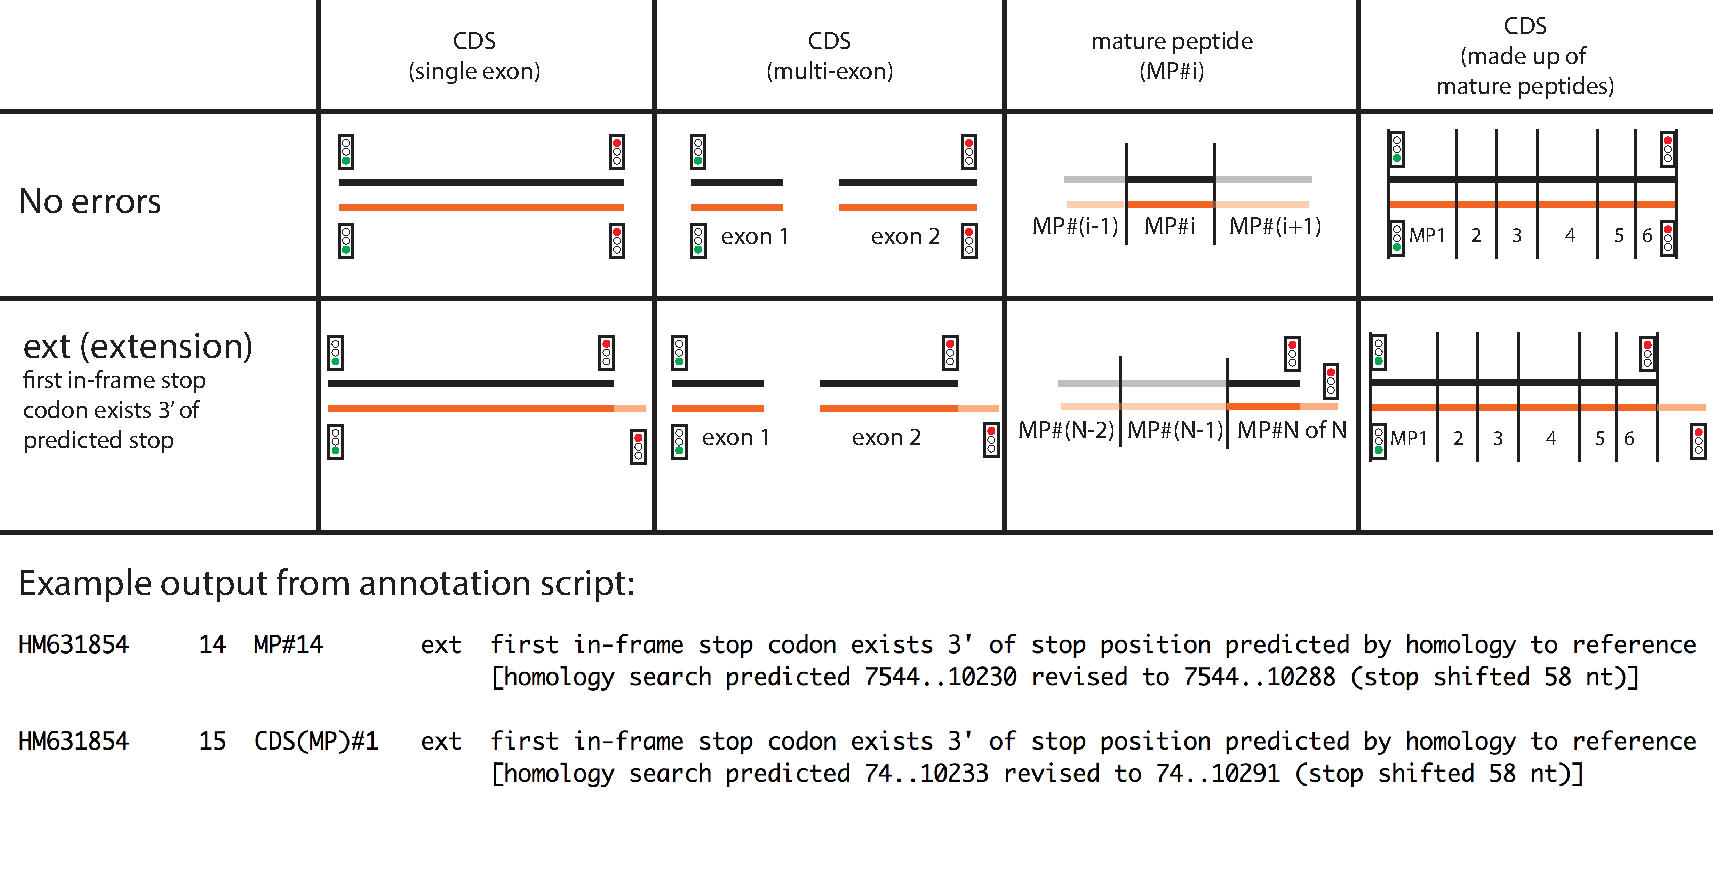
\includegraphics[width=10in]{figs/errornew-2-ext}
\end{center}
\vfill
\end{slide}
%%%%%%%%%%%%%%%%%%%%%%%%%%%%%%%%%%%%%%%%%%%%%%%%%%%%%%%%%%%%%%%%%%%%%%
\begin{slide}
\begin{center}
\textbf{olp: lack of an expected overlap with another feature}
\vspace{0.5in}

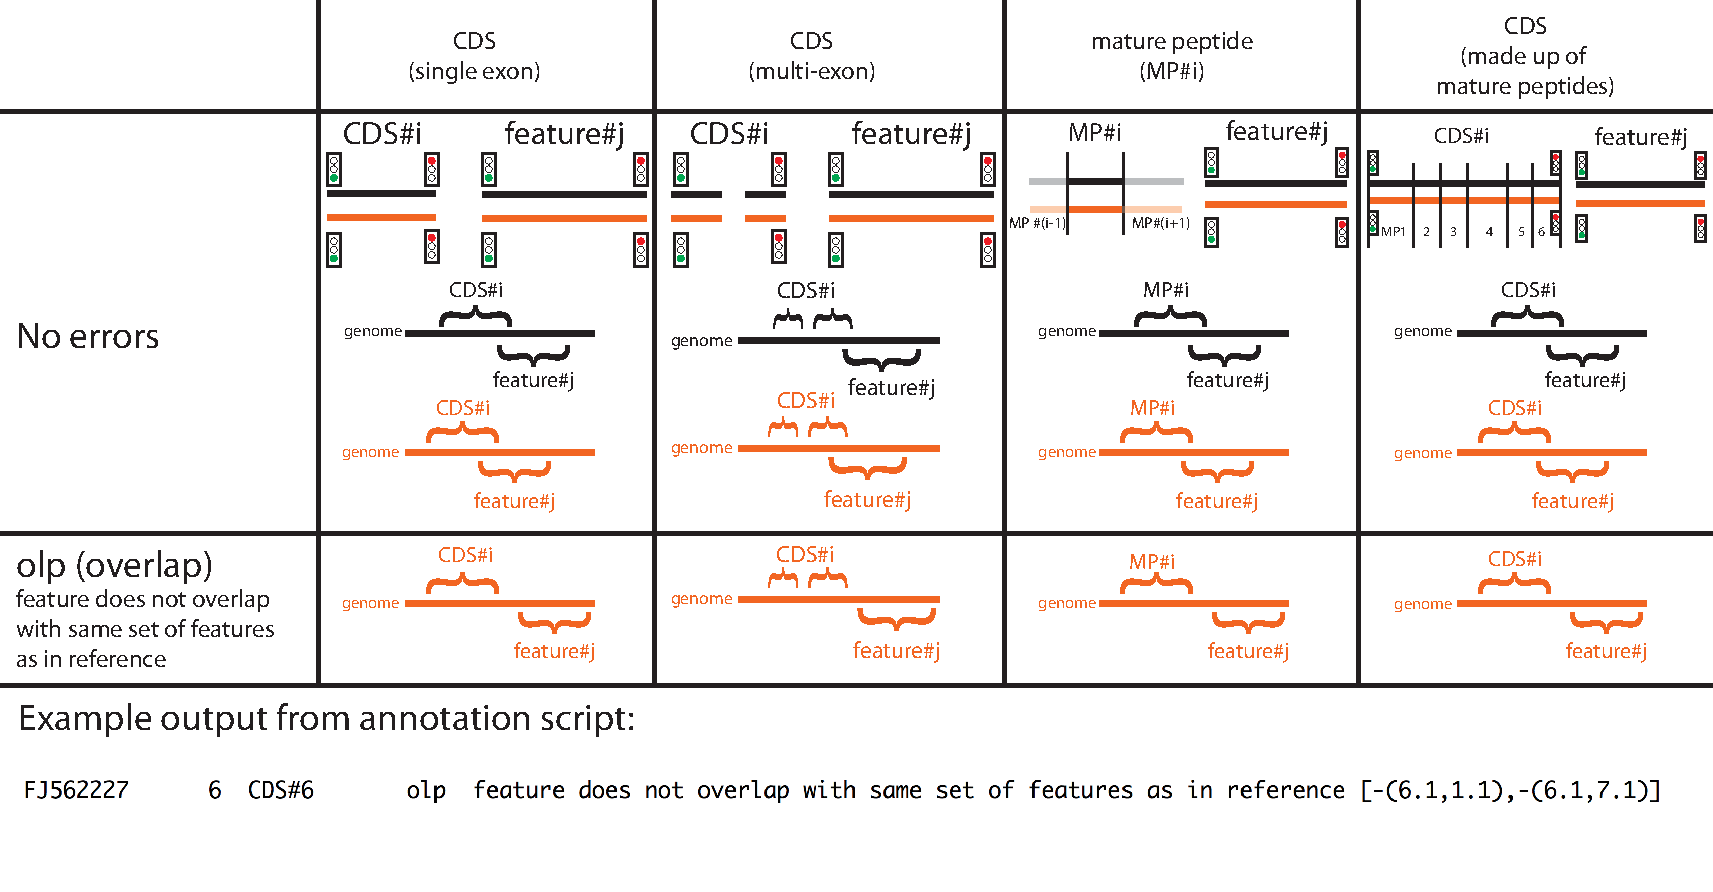
\includegraphics[width=10in]{figs/errornew-3-olp}
\end{center}
\vfill
\end{slide}
%%%%%%%%%%%%%%%%%%%%%%%%%%%%%%%%%%%%%%%%%%%%%%%%%%%%%%%%%%%%%%%%%%%%%%
\begin{slide}
\begin{center}
\textbf{ajb and aja error codes indicates lack of an expected adjacent feature}
\vspace{0.5in}

\includegraphics[width=10in]{figs/errornew-4-ajb}
\end{center}
\vfill
\end{slide}
%%%%%%%%%%%%%%%%%%%%%%%%%%%%%%%%%%%%%%%%%%%%%%%%%%%%%%%%%%%%%%%%%%%%%%
\begin{slide}
\begin{center}
\textbf{For screening submissions: mapping error codes to errors and warnings}

\small
\begin{itemize}
\item Error codes are too complex to return to submitters
\item Sometimes error codes are legitimate (true early stop)
\item Sometimes error codes reflect artefacts in the sequence (assembly error)
\item Example: trc error code leads to misc_feature and note
\end{itemize}

\includegraphics[height=3in]{figs/noro-ftable-example}

\end{center}
\vfill
\end{slide}
%%%%%%%%%%%%%%%%%%%%%%%%%%%%%%%%%%%%%%%%%%%%%%%%%%%%%%%%%%%%%%%%%%%%%%
\begin{slide}
\begin{center}
\textbf{Future directions (long term)}

\small
\begin{itemize}
%\item Annotate more species (Norovirus, Zika, and Ebola are currently \\ being checked).

%\item Long term:
\begin{itemize}
\item  Protein homology searches to supplement or replace nucleotide searches
\item  Multiple alignment (profile) based homology searches 
\item  Annotate structural RNA features (Infernal is well-suited for this)
%\item  More robust solution to the problem of finding origin sequences
\end{itemize}

%\item Short term: we have a 36 item TODO list that we agreed to with
%  J. Rodney \\ Brister's group on April 12, which includes:
%\begin{itemize}
%  \item Completed items (including analysis of West Nile annotations)
%  \item Loading and using our pipeline's annotations in the Virus Variation
%    database for Dengue and West Nile
%  \item Reviewing Ebola and Norovirus annotations
%  \item Comparing our Ebola annotations to existing annotations
%\end{itemize}
%end{itemize}

\vfill
\end{center}
\end{slide}
%%%%%%%%%%%%%%%%%%%%%%%%%%%%%%%%%%%%%%%%%%%%%%%%%%%%%%%%%%%%%%%%%%%%%%
\begin{slide}

\large
\begin{center}
\large{\textbf{Acknowledgements}} \\

\vspace{0.5in}

Alejandro Sch\"{a}ffer \\
David Landsman \\
David Lipman

\vspace{0.5in}

J. Rodney Brister \\
Ilene Mizrachi \\
Eneida Hatcher \\
Linda Yankie \\
Olga Blinkova \\
Anatoly Mnev \\
Sergey Zhdanov \\ 
Yiming Bao \\

\end{center}

\vfill
\end{slide}
%%%%%%%%%%%%%%%%%%%%%%%%%%%%%%%%%%%%%%%%%%%%%%%%%%%%%%%%%%%%%%%%%%%%%%
%%%%%%%%%%%%%%%%%%%%%%%%%%%%%%%%%%%%%%%%%%%%%%%%%%%%%%%%%%%%%%%%%%%%%%
\begin{slide}
\begin{center}
\textbf{Future directions}

\small
\begin{itemize}
\item Annotate more species (Norovirus, Zika, and Ebola are currently \\ being checked).

\item Long term:
\begin{itemize}
\item  Protein homology searches to supplement or replace nucleotide searches
\item  Given any viral sequence, find its nearest RefSeq
\item  Annotate structural RNA features (Infernal is well-suited for this)
\item  More robust solution to the problem of finding origin sequences
\item  Multiple alignment based homology searches 
\end{itemize}

\item Short term: we have a 36 item TODO list that we agreed to with
  J. Rodney \\ Brister's group on April 12, which includes:
\begin{itemize}
  \item Completed items (including analysis of West Nile annotations)
  \item Loading and using our pipeline's annotations in the Virus Variation
    database for Dengue and West Nile
  \item Reviewing Ebola and Norovirus annotations
  \item Comparing our Ebola annotations to existing annotations
\end{itemize}
\end{itemize}

\vfill
\end{center}
\end{slide}
%%%%%%%%%%%%%%%%%%%%%%%%%%%%%%%%%%%%%%%%%%%%%%%%%%%%%%%%%%%%%%%%%%%%%%
\begin{slide}
\begin{center}
\textbf{Unexpected stop codon errors (trc,ntr)}
\vspace{0.5in}

\includegraphics[width=10in]{figs/error-1-trc-ntr}
\end{center}
\vfill
\end{slide}
%%%%%%%%%%%%%%%%%%%%%%%%%%%%%%%%%%%%%%%%%%%%%%%%%%%%%%%%%%%%%%%%%%%%%%
\begin{slide}
\begin{center}
\textbf{Unexpected stop codon errors (ext,nst)}
\vspace{0.5in}

\includegraphics[width=10in]{figs/error-2-ext-nst}
\end{center}
\vfill
\end{slide}
%%%%%%%%%%%%%%%%%%%%%%%%%%%%%%%%%%%%%%%%%%%%%%%%%%%%%%%%%%%%%%%%%%%%%%
\begin{slide}
\begin{center}
\textbf{Missing expected features (str,stp,nm3)}
\vspace{0.5in}

\includegraphics[width=10in]{figs/error-3-str-stp-nm3}
\end{center}
\vfill
\end{slide}
%%%%%%%%%%%%%%%%%%%%%%%%%%%%%%%%%%%%%%%%%%%%%%%%%%%%%%%%%%%%%%%%%%%%%%
\begin{slide}
\begin{center}
\textbf{Problem with homology search prediction (bd5,bd3,nop)}
\vspace{0.5in}

\includegraphics[width=10in]{figs/error-4-bd5-bd3-nop}
\end{center}
\vfill
\end{slide}
%%%%%%%%%%%%%%%%%%%%%%%%%%%%%%%%%%%%%%%%%%%%%%%%%%%%%%%%%%%%%%%%%%%%%%
\begin{slide}
\begin{center}
\textbf{Unexpected relationship to other features (olp)}
\vspace{0.5in}

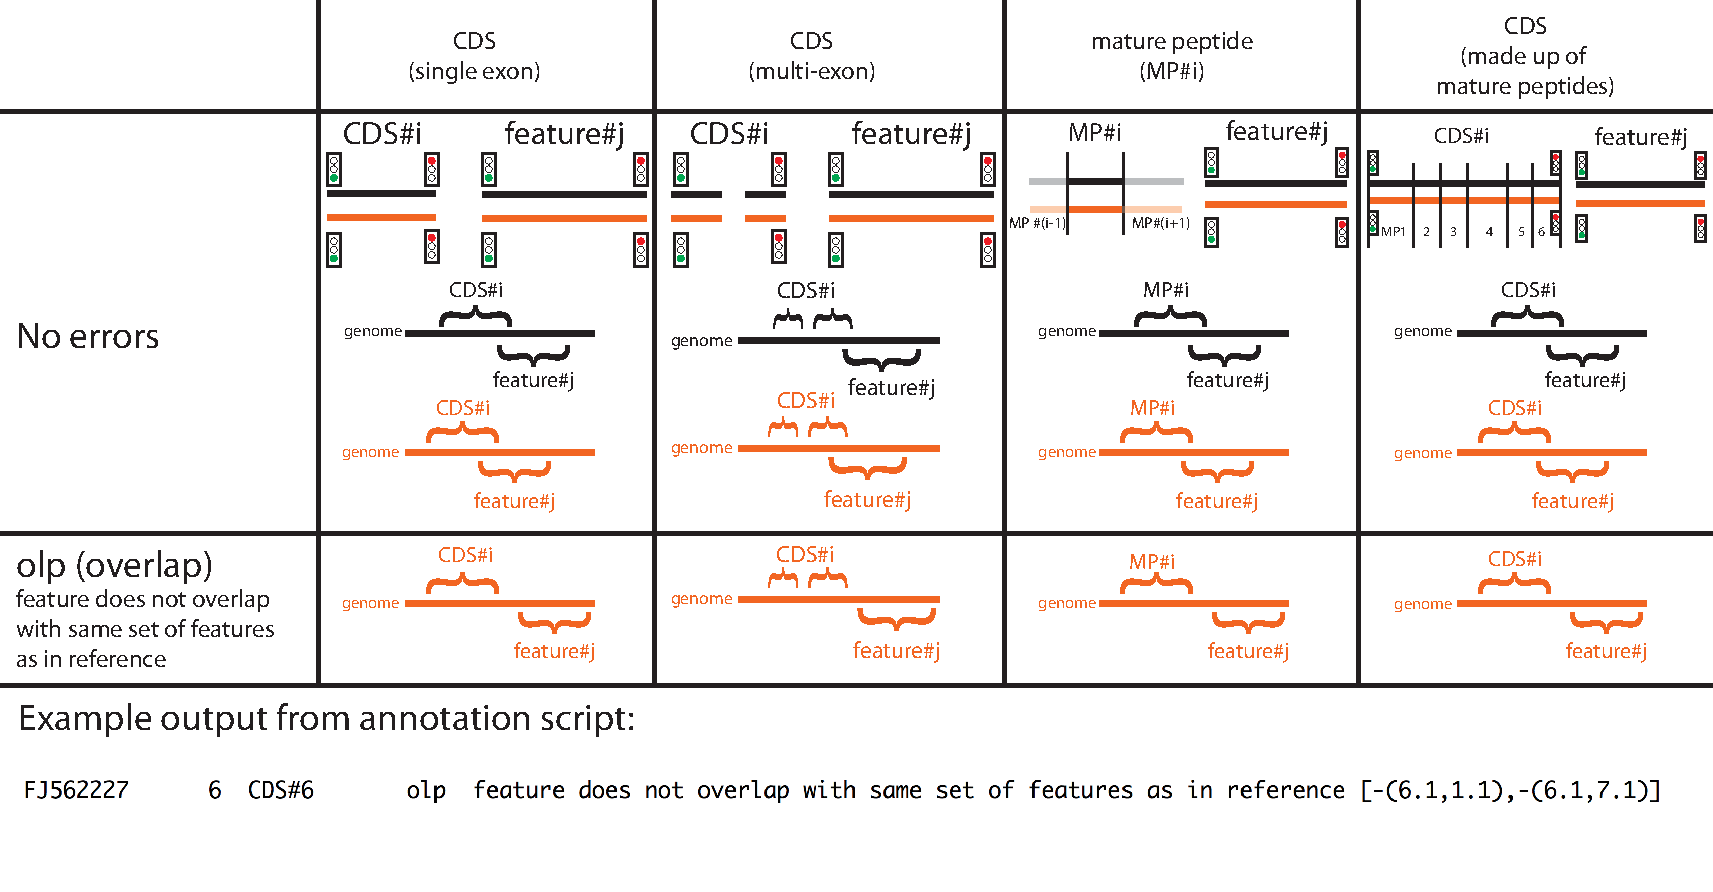
\includegraphics[width=10in]{figs/errornew-3-olp}
\end{center}
\vfill
\end{slide}
%%%%%%%%%%%%%%%%%%%%%%%%%%%%%%%%%%%%%%%%%%%%%%%%%%%%%%%%%%%%%%%%%%%%%%
\begin{slide}
\begin{center}
\textbf{Unexpected relationship to other features (ajb)}
\vspace{0.5in}

\includegraphics[width=10in]{figs/errornew-4-ajb}
\end{center}
\vfill
\end{slide}
%%%%%%%%%%%%%%%%%%%%%%%%%%%%%%%%%%%%%%%%%%%%%%%%%%%%%%%%%%%%%%%%%%%%%%
\begin{slide}
\begin{center}
\textbf{Unexpected relationship to other features (aja)}
\vspace{0.5in}

\includegraphics[width=10in]{figs/error-7-aja}
\end{center}
\vfill
\end{slide}
%%%%%%%%%%%%%%%%%%%%%%%%%%%%%%%%%%%%%%%%%%%%%%%%%%%%%%%%%%%%%%%%%%%%%%
\begin{slide}
\begin{center}
\textbf{Problem annotating CDS due to mature peptide errors (aji,int,inp)}
\vspace{0.5in}

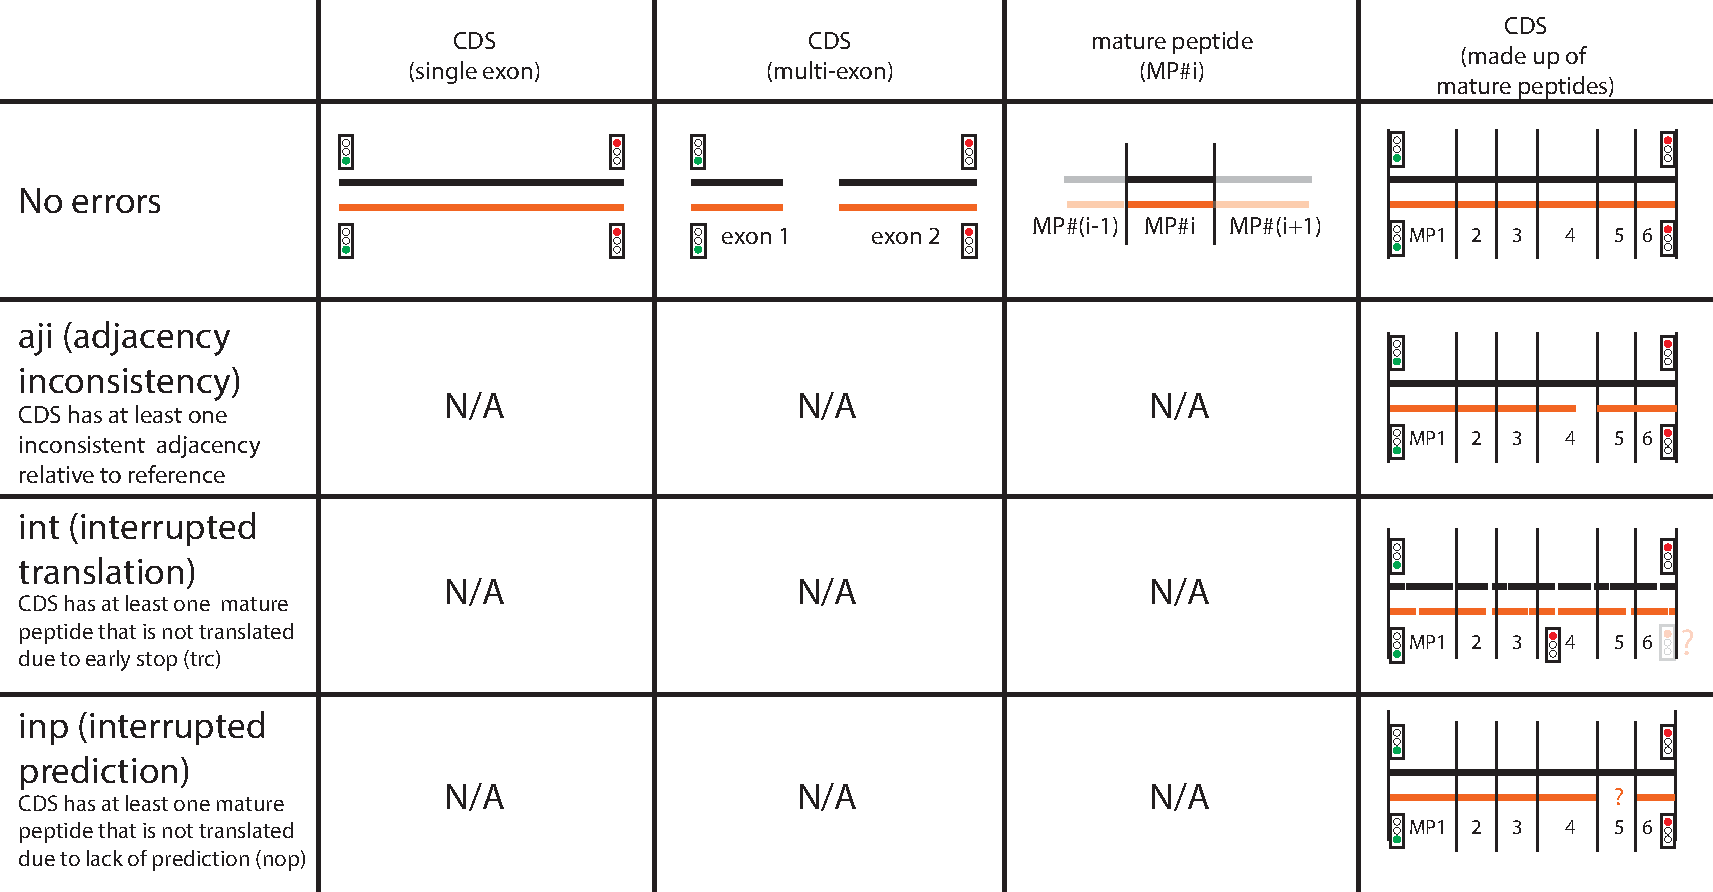
\includegraphics[width=10in]{figs/error-8-aji-int-inp}
\end{center}
\vfill
\end{slide}
%%%%%%%%%%%%%%%%%%%%%%%%%%%%%%%%%%%%%%%%%%%%%%%%%%%%%%%%%%%%%%%%%%%%%%
\begin{slide}
\begin{center}
\textbf{Lack of exactly one origin sequence (ori)}
\vspace{0.5in}

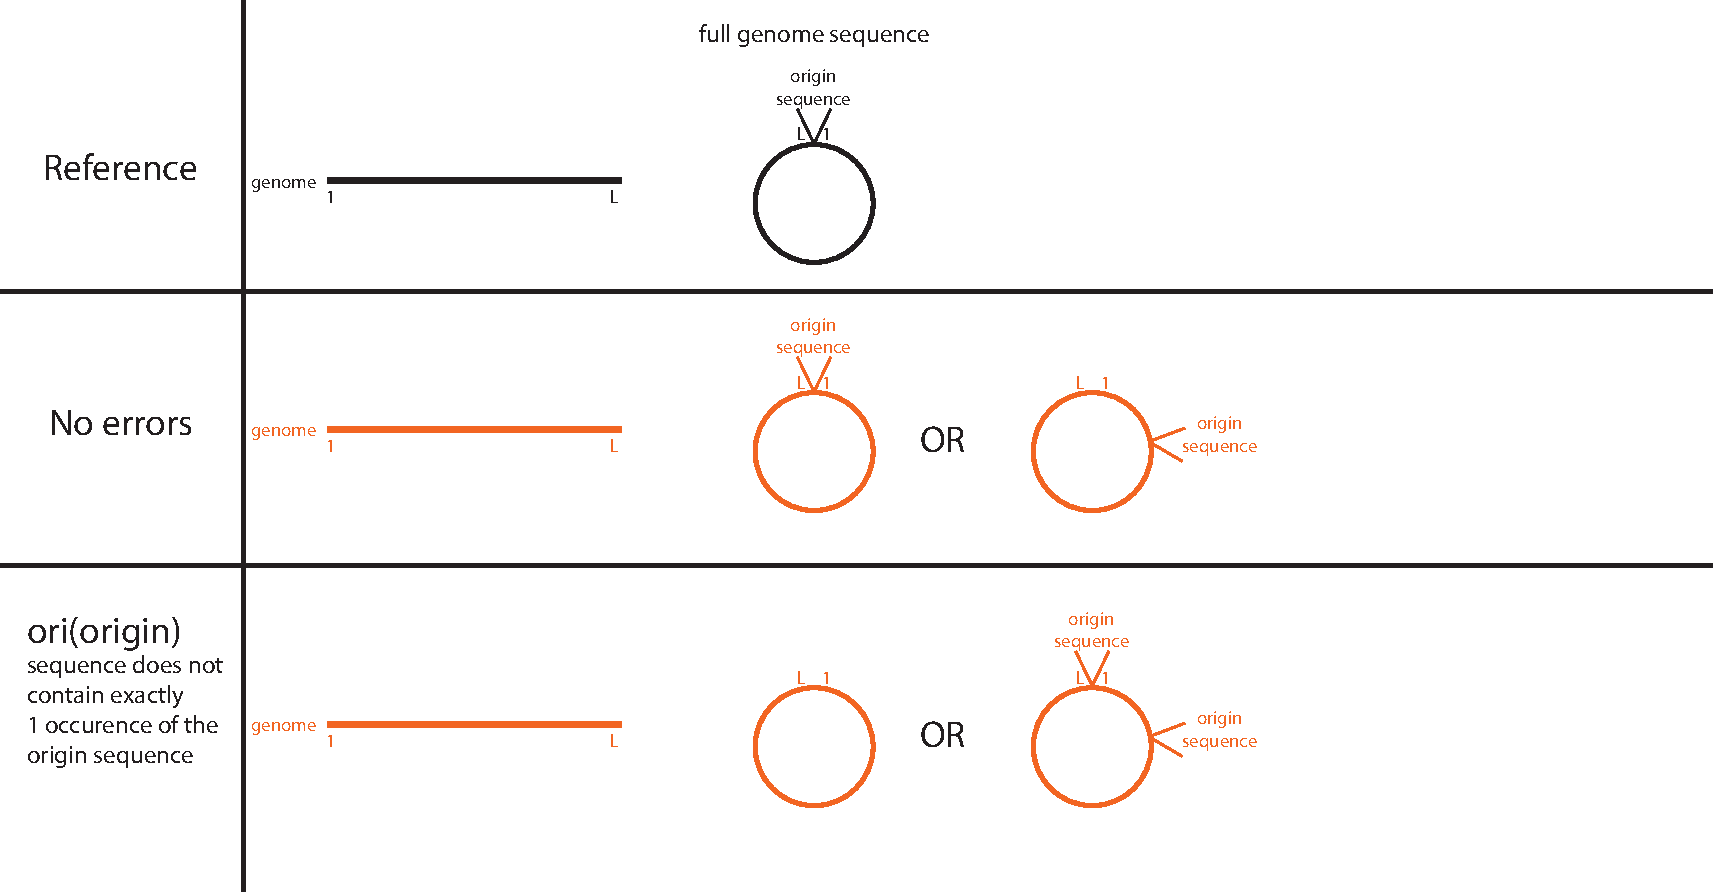
\includegraphics[width=10in]{figs/error-9-ori}
\end{center}
\vfill
\end{slide}
%%%%%%%%%%%%%%%%%%%%%%%%%%%%%%%%%%%%%%%%%%%%%%%%%%%%%%%%%%%%%%%%%%%%%%

\end{document}
